\documentclass{article}
\usepackage{amsmath}
\usepackage{graphicx}
\begin{document}
\title{Coordinate Geometry Unit Exam: Question 40}
\author{Ana Bhattacharjee}
\date{\today}
\maketitle{}

\begin{center}
The image of the circle is shown below.
\begin{figure}[!htbp]
  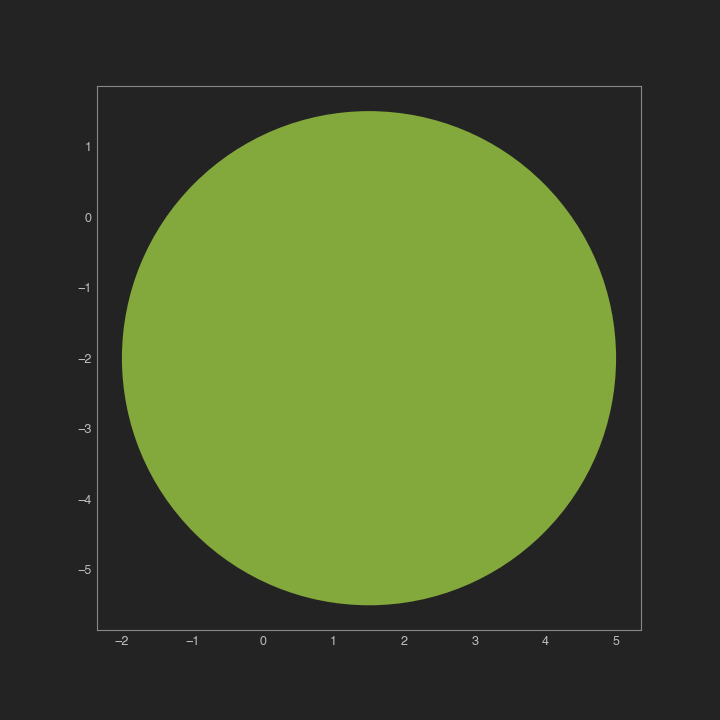
\includegraphics[width=1.0\columnwidth]{circle}
  \caption{Circle}
\end{figure}
\par
The first step is to find the radius. We are given the terminii of the diameter so let's compute the distance first and then we'll divide it by two to get the radius.
\begin{align}
  d = \sqrt{(x_2 - x_1)^2 + (y_2 - y_1)^2} \\
  d = \sqrt{(-4 - 3)^2 + (0 - 0)^2} \rightarrow \sqrt{(49)} = 7 \\
  r = d / 2 = 3.5
\end{align}
Now we need to find the center of the circle. The center is essentially the midpoint of the diameter.
\begin{align}
  M = (\frac{x_1 + x_2}{2}, \frac{y_1 + y_2}{2}) \\
  M = (\frac{3 + -4}{2}, \frac{0 + 0 }{2}) \\
  M = (\frac{-1}{2}, 0)
\end{align}
With the above information, we can now create the equation of the circle.
\begin{align}
  (x + \frac{1}{2})^2 + y^2 = 49 
\end{align}
\end{center}
\end{document}
